\subsection{Retourner la réponse textuelle sous la forme d'un signal audio}
Une fois une réponse générée, il est intéressant de générer l’audio de cette à nouveau afin de répondre à l’utilisateur, ce qui est un autre calcul rapide qui peut se faire en temps réel. Cela est possible avec le CNN (Conv.. neural net) Wavenet d’Aaron van den Oord et al., développé chez Google \cite{wavenet}. En effet, il est possible de générer n’importe quel ton de voix avec \texttt{Wavenet}, ainsi le choix de la voix de la personne qui parle peut être fait par l’utilisateur. À titre d’exemple, cette architecture neurale est tellement puissante qu’il est possible de lui faire imiter la voix du président. Cette découverte récente par Google est la première fois qu’il est possible de confondre la voix pour une voix humaine réelle plutôt qu’une voix robotique, ainsi l’illusion est bien réussie. La façon dont \texttt{Wavenet} fonctionne est d’établir un préalable statistique (une variable conditionnée) qui est donnée à un premier algorithme qui s’occupe de trouver les bons tons de voix à générer avec \texttt{Wavenet}, à partir du texte. C’est ainsi que Wavenet, conditionné lui-même par le ton de voix demandé et par le texte, peut générer la voix de façon réalistique. C’est une méthode point par point, ainsi, chaque point dans la vague audio est généré en fonction des points précédents et du conditionnement demandé, c’est très bas niveau sur le signal qui est à un taux d’échantillonage de 16 kHz lors de l’entraînement, ce qui est assez pour capturer les subtilités de quelqu’un qui parlerait réellement dans un enregistrement. Cette phase générative est illustrée dans dans la \autoref{fig:wavenet}.

\begin{figure*}
  \centering
  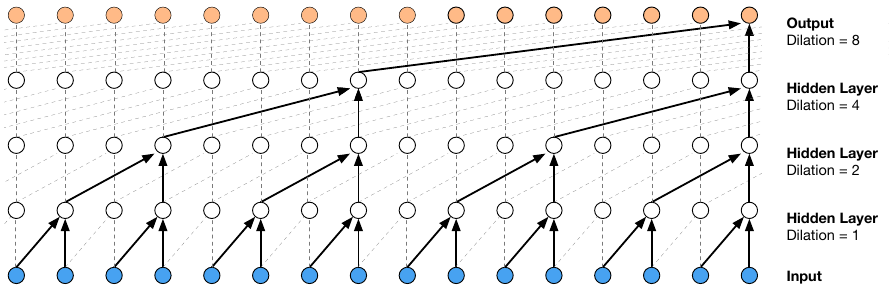
\includegraphics[width=\textwidth]{wavenet}
  \caption{À l’aide de convolutions causales dilatées, il est possible de prédire le prochain point dans la vague audio de façon efficace. Cela est un modèle autorégréssif : les points passés sont utilisés pour prédire les points suivants du même signal. Ainsi, la sortie est remise en entrée pour le calcul de l’étape suivante, ce sampling peut faire usage de mémoire cache, ce qui donne à cet algorithme générationnel un temps linéaire pour la génération, cela en fonction de la longueur du signal à générer \cite{wavenet}.}
  \label{fig:wavenet}
\end{figure*}
